\documentclass[A4paper,]{article}
\usepackage{lmodern}
\usepackage{amssymb,amsmath}
\usepackage{ifxetex,ifluatex}
\usepackage{fixltx2e} % provides \textsubscript
\ifnum 0\ifxetex 1\fi\ifluatex 1\fi=0 % if pdftex
  \usepackage[T1]{fontenc}
  \usepackage[utf8]{inputenc}
\else % if luatex or xelatex
  \ifxetex
    \usepackage{mathspec}
  \else
    \usepackage{fontspec}
  \fi
  \defaultfontfeatures{Ligatures=TeX,Scale=MatchLowercase}
\fi
% use upquote if available, for straight quotes in verbatim environments
\IfFileExists{upquote.sty}{\usepackage{upquote}}{}
% use microtype if available
\IfFileExists{microtype.sty}{%
\usepackage{microtype}
\UseMicrotypeSet[protrusion]{basicmath} % disable protrusion for tt fonts
}{}
\usepackage[margin=3.7cm]{geometry}
\usepackage[unicode=true]{hyperref}
\hypersetup{
            pdftitle={Generative spaces: assisting the level designer in creating world maps},
            pdfauthor={Pedro Caldeira},
            pdfborder={0 0 0},
            breaklinks=true}
\urlstyle{same}  % don't use monospace font for urls
\usepackage{graphicx,grffile}
\makeatletter
\def\maxwidth{\ifdim\Gin@nat@width>\linewidth\linewidth\else\Gin@nat@width\fi}
\def\maxheight{\ifdim\Gin@nat@height>\textheight\textheight\else\Gin@nat@height\fi}
\makeatother
% Scale images if necessary, so that they will not overflow the page
% margins by default, and it is still possible to overwrite the defaults
% using explicit options in \includegraphics[width, height, ...]{}
\setkeys{Gin}{width=\maxwidth,height=\maxheight,keepaspectratio}
\IfFileExists{parskip.sty}{%
\usepackage{parskip}
}{% else
\setlength{\parindent}{0pt}
\setlength{\parskip}{6pt plus 2pt minus 1pt}
}
\setlength{\emergencystretch}{3em}  % prevent overfull lines
\providecommand{\tightlist}{%
  \setlength{\itemsep}{0pt}\setlength{\parskip}{0pt}}
\setcounter{secnumdepth}{5}
% Redefines (sub)paragraphs to behave more like sections
\ifx\paragraph\undefined\else
\let\oldparagraph\paragraph
\renewcommand{\paragraph}[1]{\oldparagraph{#1}\mbox{}}
\fi
\ifx\subparagraph\undefined\else
\let\oldsubparagraph\subparagraph
\renewcommand{\subparagraph}[1]{\oldsubparagraph{#1}\mbox{}}
\fi

% set default figure placement to htbp
\makeatletter
\def\fps@figure{htbp}
\makeatother

\usepackage{graphicx}
\usepackage{mathtools}
\usepackage{tikz}
\usepackage{subfig}
\AtBeginDocument{%
\renewcommand*\figurename{Figure}
\renewcommand*\tablename{Table}
}
\AtBeginDocument{%
\renewcommand*\listfigurename{List of Figures}
\renewcommand*\listtablename{List of Tables}
}
\usepackage{float}
\floatstyle{ruled}
\makeatletter
\@ifundefined{c@chapter}{\newfloat{codelisting}{h}{lop}}{\newfloat{codelisting}{h}{lop}[chapter]}
\makeatother
\floatname{codelisting}{Listing}
\newcommand*\listoflistings{\listof{codelisting}{List of Listings}}

\title{Generative spaces: assisting the level designer in creating world maps}
\author{Pedro Caldeira}
\date{}

\begin{document}
\maketitle
\begin{abstract}
Creating two-dimensional tile maps by hand is a long and tedious
process. Tile maps contain an inherent structure and repetition that we
should be able to exploit. We provide a way of generating these maps
automatically using machine learning techniques. With these set of tools
level designers will be able to create worlds that are much larger in
scope.
\end{abstract}

\section{Introduction}\label{introduction}

The development of a video game requires a great variety of assets. A
typical game combines music, art and code to form a coherent whole.

This need for resources is one of the reasons why games are so costly to
develop. Procedural content generation---the automatic creation of
content---has emerged as an answer to this problem and is currently
widely used, particularly in studios with few resources. For example,
\emph{No Man's Sky (2016)} is a space exploration game that uses
procedural generation to generate a whole universe of over 18
quintillion planets \(1.8 \cdot 10^{19}\), suffice to say that you would
need many lifetimes to explore them all.

Most approaches to procedural generation are rule based, meaning that
they rely on the definition of explicit rules. L-systems (Lindenmayer
1968) are an example of such a rule based system, which allows the
creation of tree-like structures. The limitations of rule based systems
lies in the fact that they cannot learn from already existing examples
and reproduce them. We would not be able to show an L-system images of
oaks for example and expect it to reproduce trees in the same style. We
would need to define exactly the rules that represent ``oakness'', the
attributes give rise to the distinct features of the oak.

Data-driven techniques for procedural generation are still relatively
rare; in this paper we try to see whether it is possible to reproduce
the spatial style of a given game using data-driven techniques.

\begin{itemize}
\item
  We show how 2d Markov chains can be applied to the generation of 2d
  tile-maps that are non-linear in nature. As opposed to past
  litterature (Snodgrass and Ontañón 2013) we use maps with a larger
  number of tile types. Section \ref{sec:background} provides a few
  background information on what tile-maps are and their current uses
  while Section \ref{sec:markov-chains} describes the technical side of
  2d Markov chains.
\item
  We argue that the generated maps keep the spatial style of the
  originals by comparing how different input maps influence the
  generated maps in Section \ref{sec:spatial-style}.
\item
  We come up with a backoff smoothing method appropriate for 2d chains.
  First we explain why it can be useful in Section \ref{sec:idea} and
  then we give the technical details of its implementation in Section
  \ref{sec:backoff}.
\item
  We provide a C\# implementation of a text based 2d Markov chain which
  is accessible at the following link\footnote{https://github.com/stonecauldron/markov2d}.
\end{itemize}

\section{Background}\label{sec:background}

First of all let us define more precisely what a tile-map is. Tile-maps
are a staple of many genres of games, they are formed by individual
tiles of predefined size and assembled into a grid.

\begin{figure}
\centering
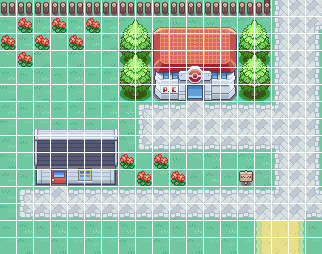
\includegraphics[width=0.75000\textwidth]{img/tile-map-example.png}
\caption{An example of a tile-map with the grid structure visible.\\
\emph{Pokemon FireRed (2004)}}
\end{figure}

Game developers make use of tile-maps for various reasons:

\begin{itemize}
\tightlist
\item
  They reduce the number of art assets that need to be created for the
  game since the same tile can be reused in multiple places.
\item
  Levels created with tile-maps can be easily represented in a digital
  format; we can represent them as a matrix where each entry contains a
  tile identifier.
\item
  They allow the level designer to create new levels without having to
  worry about creating new art assets. In some cases this can be
  extended into fully-fledged level editors where the players themselves
  can create new levels\footnote{A striking example is the game
    \emph{Super Mario Maker} which is built entirely around the concept
    of players creating \emph{Mario Bros.} levels.}.
\item
  They permit the separation of gameplay and visual appearance. Tiles
  can for example represent non-traversable and empty space
  independently from their look in-game.
\end{itemize}

Traditionally tile-maps are built manually: the level designer chooses
one tile for each cell of the grid. Given that the grids can be very
large, we can easily imagine that this is a time-consuming process. It
puts a human limit into the size of the maps that can be used in a game.
Being able to generate these maps procedurally would lift a burden off
the shoulders of the level designers and allow the generation of much
larger worlds.

The use of tile-maps might seem like an outdated method but they are
still used in many independent games, some of which have been quite
successful\footnote{\emph{Stardew Valley (2016)} or \emph{Undertale
  (2015)} are both million seller games that make use of tile-maps.}.

\section{The idea}\label{sec:idea}

Let us remind you of our objective; we want to be able to generate
tile-maps from a set of representative examples. Our process has the
following steps:

\begin{enumerate}
\def\labelenumi{\arabic{enumi}.}
\tightlist
\item
  We choose the set of maps whose spatial style we want to reproduce.
\item
  We represent the maps as matrices where each entry contains a tile
  type identifier. This will be our input dataset.
\item
  We generate a Markov chain whose probability distributions reflect
  those of the original dataset. This is the learning phase of the
  model.
\item
  We then sample this Markov chain to generate a map of any given
  dimension.
\end{enumerate}

This is comparable to the case where Markov chains are used for
automatic essay writing (Murphy 2012). These automatically written
essays use similar idioms and vocabulary to the ones present in the
learning dataset; in a certain sense they emulate the style of a given
text. For the same reasons we expect our Markov chains to reproduce the
spatial style of its learning examples.

One of the problems that appears when sampling Markov chains is that is
likely for a chain to generate a sequence of elements that do not exist
in the training dataset. As an example take the word predictors that are
present in most mobile phones today; Imagine you have just typed the
words ``Colorless green ideas sleep''\footnote{This sentence is an
  example of a grammatically correct sentence with no meaning which we
  can assume does not occur in a standard English text. Taken from
  Chomsky 1956}, since this sentence is not present in the training
corpus, the Markov chain will not be able to infer what the next most
probable word is and will have to stop generating text.

A way of solving this problem is to use what is called backoff smoothing
(Murphy 2012) in which we consider less elements of the chain when faced
with unknown data. To take our above example again, instead of
considering the whole chain to infer the next most likely word we can
restrict ourselves to the previous word only, which in this case is
``sleep''. By reducing the number of elements we consider in the chain,
we increase the chances of finding equivalent sequences in the training
data, thus improving the robustness of the model.

While the definition of backoff smoothing is simple with linear chains,
it becomes more complicated in the case of 2d chains. Our approach is
detailed in Section \ref{sec:backoff}.

\section{Results}\label{results}

In this section we will try to evaluate qualitatively a set of maps
generated with our method. To this end we will use data from the game
\emph{Pokemon Red (1996)} and \emph{Pokemon FireRed (2004)}. The
\emph{FireRed} version is a remake of the \emph{Red} version meaning
that is mainly a visual upgrade of the first game; the locations and the
spatial distribution of both games are very similar. This allows us to
see first hand the effects of an increase in the number of unique tiles:
\emph{Pokemon Red} has 125 unique tiles while \emph{Pokemon FireRed} has
1207 different tiles.

\begin{figure}
\centering
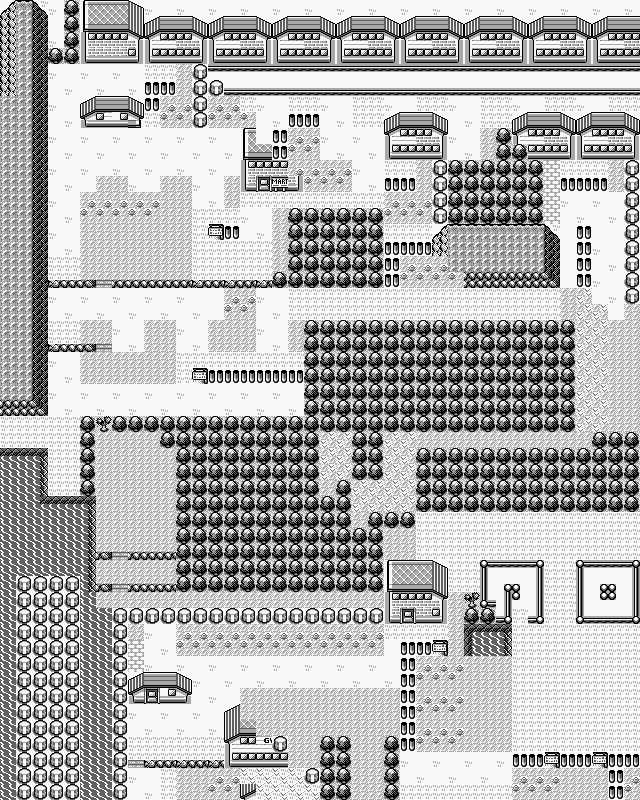
\includegraphics[width=0.50000\textwidth]{../data/pokemon-red/generated/100n-3k/image/46.png}
\caption{A generated map based on \emph{Pokemon
Red}}\label{fig:red-result}
\end{figure}

\begin{figure}
\centering
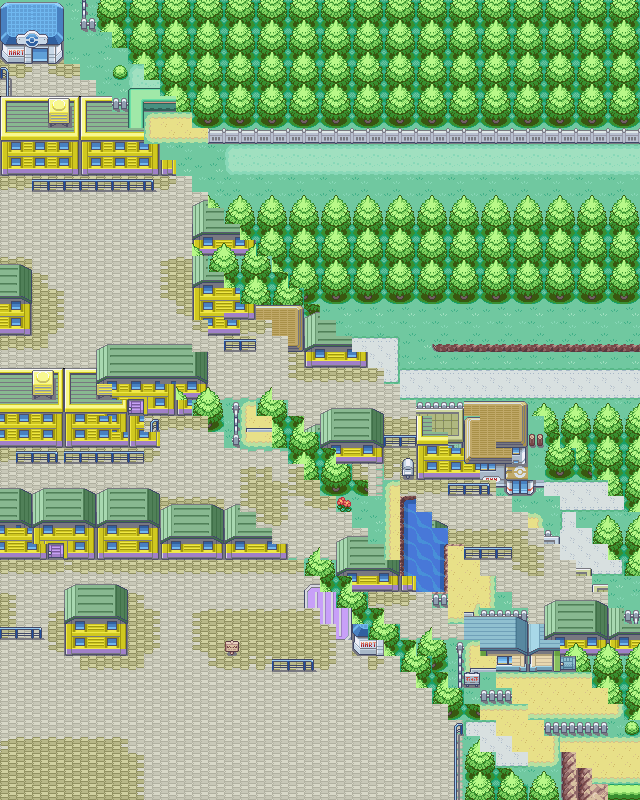
\includegraphics[width=0.50000\textwidth]{../data/pokemon-firered/generated/250n-3k/image/35.png}
\caption{A generated map based on \emph{Pokemon
FireRed}}\label{fig:firered-result}
\end{figure}

In the \emph{Red} version (fig.~\ref{fig:red-result}) the overall
results looks quite promising:

\begin{itemize}
\tightlist
\item
  Except a patch of grass in the center, almost all the navigable space
  in the map is reachable.
\item
  Aesthetically the map is plausible; it is comparable to what we can
  find in the original \emph{Pokemon Red} game with a similar
  distribution of tiles.
\item
  There are few incomplete structures in the map, mainly the buildings.
  This is due to the fact that they are the structures with the largest
  number of dependencies in the tiles that compose them.
\end{itemize}

In \emph{FireRed} (fig.~\ref{fig:firered-result}) the result is much
worse though, there is a much larger number of incomplete structures and
while the map looks believable locally, the transition between a forest
environment and a city environment in the diagonal is problematic.

This is due to the following facts:

\begin{itemize}
\tightlist
\item
  The \emph{FireRed} version has a higher number of tiles that do not
  make sense when they are taken individually. The trees in
  \emph{FireRed} for example are composed of multiple tiles while in
  \emph{Red} they take up only one tile.
\item
  \emph{FireRed} uses many tiles that have similar meaning but different
  appearances. The visual look of houses in \emph{FireRed} are very
  varied while in \emph{Red} they are much more homogeneous.
\item
  The problem on the diagonal suggests that there is not enough data for
  transitions between different environments. The diagonal shape is due
  to the ways the backoff smoothing works: in this case it has not
  enough data to generate the tiles and must rely only on the diagonal
  predecessors to generate the next tile.
\end{itemize}

These problems come from the fact that the dependencies between the map
elements have a farther reach than what can appropriately be captured by
the method. This lead us to believe that to work on games with large
tilesets we would need a higher amount of data. Alternatively a few
possible improvements to the method are discussed in Section
\ref{sec:conclusion}.

The computational complexity of our method is linear in relation to the
map size for both training and generation.\footnote{This remains true as
  long as we assume to take a relatively small number of predecessors
  into account. See Section \ref{sec:backoff} for more details.} This
implies we can imagine using the method to generate maps dynamically
providing players with new levels at each playthrough.

\section{Technical details}\label{technical-details}

\subsection{2d Markov chains}\label{sec:markov-chains}

Markov chains are a mathematical formalism that allows us to model state
transitions of a stochastic process. The particularity of Markov chains
is that they only take the current state of the system into account to
compute the next state. We can for example model the weather by two
states: \emph{sunny} and \emph{rainy} and define that the probabilities
of the weather being either sunny or rainy the next day only depend on
the current weather.

In our use case we represent a tile-map as a matrix where each entry
corresponds to a specific tile. The Markov chain generating the map will
have one state per tile type and will fill the matrix of the tile-map
sequentially by sampling the next state at each entry.

The chains are trained on the example data with a frequency computation.
We used the approach that is detailed in Snodgrass and Ontañón (2013).

This assumption that the next state only depends on the current state is
called the \emph{Markov property}. This property can be extended to hold
on any number of previous states of the system, in which case we talk
about higher order Markov chains. We can even assume that the
predecessors are not only linear but that they are taken in multiple
dimensions.

\begin{figure}[h]
\centering
\begin{tikzpicture}[scale=0.2]
\tikzstyle{every node}+=[inner sep=0pt]
\draw [black] (7.7,-6.6) circle (3);
\draw (7.7,-6.6) node {$S_{1,1}$};
\draw [black] (18.3,-6.6) circle (3);
\draw (18.3,-6.6) node {$S_{1,2}$};
\draw [black] (28.8,-6.6) circle (3);
\draw (28.8,-6.6) node {$S_{1,3}$};
\draw [black] (7.7,-15.8) circle (3);
\draw (7.7,-15.8) node {$S_{2,1}$};
\draw [black] (18.3,-15.8) circle (3);
\draw (18.3,-15.8) node {$S_{2,2}$};
\draw [black] (28.8,-15.8) circle (3);
\draw (28.8,-15.8) node {$S_{2,3}$};
\draw [black] (39,-6.6) circle (3);
\draw (39,-6.6) node {$...$};
\draw [black] (39,-15.8) circle (3);
\draw (39,-15.8) node {$...$};
\draw [black] (7.7,-24.8) circle (3);
\draw (7.7,-24.8) node {$...$};
\draw [black] (18.3,-24.8) circle (3);
\draw (18.3,-24.8) node {$...$};
\draw [black] (28.8,-24.8) circle (3);
\draw (28.8,-24.8) node {$...$};
\draw [black] (7.7,-9.6) -- (7.7,-12.8);
\fill [black] (7.7,-12.8) -- (8.2,-12) -- (7.2,-12);
\draw [black] (10.7,-6.6) -- (15.3,-6.6);
\fill [black] (15.3,-6.6) -- (14.5,-6.1) -- (14.5,-7.1);
\draw [black] (21.3,-6.6) -- (25.8,-6.6);
\fill [black] (25.8,-6.6) -- (25,-6.1) -- (25,-7.1);
\draw [black] (10.7,-15.8) -- (15.3,-15.8);
\fill [black] (15.3,-15.8) -- (14.5,-15.3) -- (14.5,-16.3);
\draw [black] (21.3,-15.8) -- (25.8,-15.8);
\fill [black] (25.8,-15.8) -- (25,-15.3) -- (25,-16.3);
\draw [black] (18.3,-9.6) -- (18.3,-12.8);
\fill [black] (18.3,-12.8) -- (18.8,-12) -- (17.8,-12);
\draw [black] (28.8,-9.6) -- (28.8,-12.8);
\fill [black] (28.8,-12.8) -- (29.3,-12) -- (28.3,-12);
\draw [black] (7.7,-18.8) -- (7.7,-21.8);
\fill [black] (7.7,-21.8) -- (8.2,-21) -- (7.2,-21);
\draw [black] (18.3,-18.8) -- (18.3,-21.8);
\fill [black] (18.3,-21.8) -- (18.8,-21) -- (17.8,-21);
\draw [black] (28.8,-18.8) -- (28.8,-21.8);
\fill [black] (28.8,-21.8) -- (29.3,-21) -- (28.3,-21);
\draw [black] (10.7,-24.8) -- (15.3,-24.8);
\fill [black] (15.3,-24.8) -- (14.5,-24.3) -- (14.5,-25.3);
\draw [black] (21.3,-24.8) -- (25.8,-24.8);
\fill [black] (25.8,-24.8) -- (25,-24.3) -- (25,-25.3);
\draw [black] (31.8,-6.6) -- (36,-6.6);
\fill [black] (36,-6.6) -- (35.2,-6.1) -- (35.2,-7.1);
\draw [black] (31.8,-15.8) -- (36,-15.8);
\fill [black] (36,-15.8) -- (35.2,-15.3) -- (35.2,-16.3);
\draw [black] (39,-9.6) -- (39,-12.8);
\fill [black] (39,-12.8) -- (39.5,-12) -- (38.5,-12);
\end{tikzpicture}
\caption{A figure showing the dependencies in a 2d Markov chain}
\end{figure}

The number and position of previous tiles that are taken into account
are explicitly defined by the predecessors matrix.

\begin{figure}[h]
\centering
$
P_1=
\begin{pmatrix}
 0& 1& 0\\ 
 0& 0& 0\\ 
 0& 0& 0 
\end{pmatrix}
$
$
P_2= 
\begin{pmatrix}
 0& 0& 0\\ 
 1& 0& 0\\ 
 0& 0& 0 
\end{pmatrix}
$
$
P_3=
\begin{pmatrix}
 0& 1& 1\\ 
 1& 1& 1\\ 
 1& 1& 1 
\end{pmatrix}
$
\caption{Various predecessors matrices: $P_1$ only takes into account the
nearest left neighbour, $P_2$ only the nearest upper neighbour and $P_3$ takes
all neighbours that are at a distance of 3 or less of the current tile.}
\end{figure}

\begin{figure}
\centering
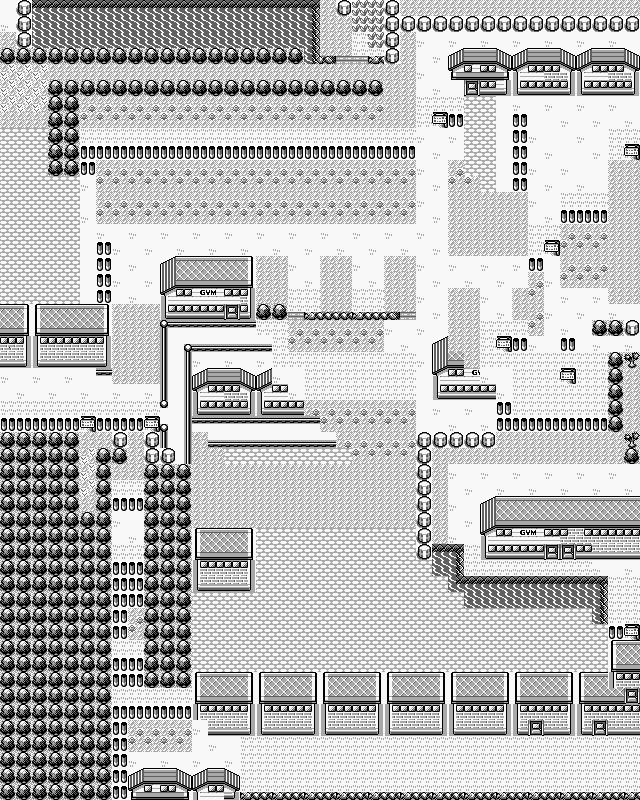
\includegraphics[width=0.50000\textwidth]{../data/pokemon-red/generated/250n-3k/image/36.png}
\caption{A map generated with predecessor matrix
\(P_3\)}\label{fig:3k-map}
\end{figure}

\begin{figure}
\centering
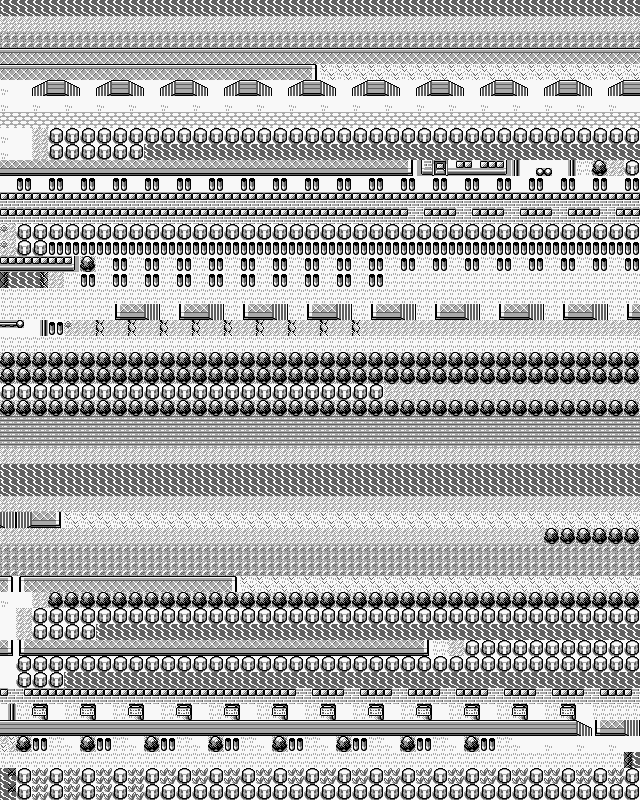
\includegraphics[width=0.50000\textwidth]{../data/pokemon-red/generated/250n-1k/image/7.png}
\caption{A map generated with predecessor matrix
\(P_1\)}\label{fig:1k-map}
\end{figure}

As we can see in fig.~\ref{fig:3k-map} and fig.~\ref{fig:1k-map} the
choice of the predecessor has a big influence on the outcome of the
generation. In fig.~\ref{fig:1k-map} each tile takes only its immediate
left neighbour into account, the chain is linear and we can easily see
that there are no relations between each rows. In fig.~\ref{fig:3k-map}
we use a predecessors matrix that is two-dimensional and we can
immediately see that the generated map produced much more complex
spatial structures as evidenced by the presence of elements composed by
a combination of tiles such as houses and buildings.

In general, larger predecessor matrices allow the expression of more
complex structures, their use however is limited by the fact that they
require more data to train. Imagine we take a predecessor matrix of the
size of the training maps, then the trained Markov chain would only be
able to generate copies of its training data since it has not learned
anything else. We thus lose the potential for variability in the maps
generated with larger predecessor matrices.

\subsection{Spatial style conservation}\label{sec:spatial-style}

For our approach to be valid, the generated maps must reproduce the
spatial style that is present in the training data-set. If this
assumption is true then we expect that if we take two different games as
training data that the generated maps will be different not only in the
aesthetic sense but also in the spatial sense. As we said in Section
\ref{sec:background} we can associate each tile with spatial meaning by
defining if it is traversable by the player or not. We can then
represent the tile-maps with only two tile types:

\begin{itemize}
\tightlist
\item
  A tile representing empty space depicted as a black tile.
\item
  A tile representing an obstacle depicted as a white tile.
\end{itemize}

To this end we generate two tile-maps with different games as training
data; in fig.~\ref{fig:mario-binary} we use levels from \emph{Mario} as
training data and in fig.~\ref{fig:red-binary} we use use training data
from \emph{Pokemon}. We can immediately notice differences in the
structure of the maps:

\begin{itemize}
\tightlist
\item
  The empty space in the \emph{Mario} map is almost all concentrated in
  the upper part of the level. This is to give the player room to jump
  and traverse the obstacles of the level. In the \emph{Pokemon} map
  however the empty space is much more dispersed; this can be explained
  by the fact that the player can navigate in two-dimensions.
\item
  We can clearly see a ground-like structure in the bottom of the
  \emph{Mario} level and a few airborne platforms while the distribution
  of the obstacles in the \emph{Pokemon} map is much more varied.
\end{itemize}

The differences in these binary maps can be attributed to the way the
players navigate space in their respective games. In \emph{Mario} the
player moves through the levels in a left to right direction avoiding
enemies and obstacles by jumping; the levels have only one direction of
progression. In contrast to the \emph{Mario} games, in \emph{Pokemon}
the players can freely move with two degrees of freedom, the progression
is non-linear and much less constrained. Given these differences in the
generated maps we can assume the Markov chains do succeed in reproducing
the spatial style of their training data.

\begin{figure}
\centering
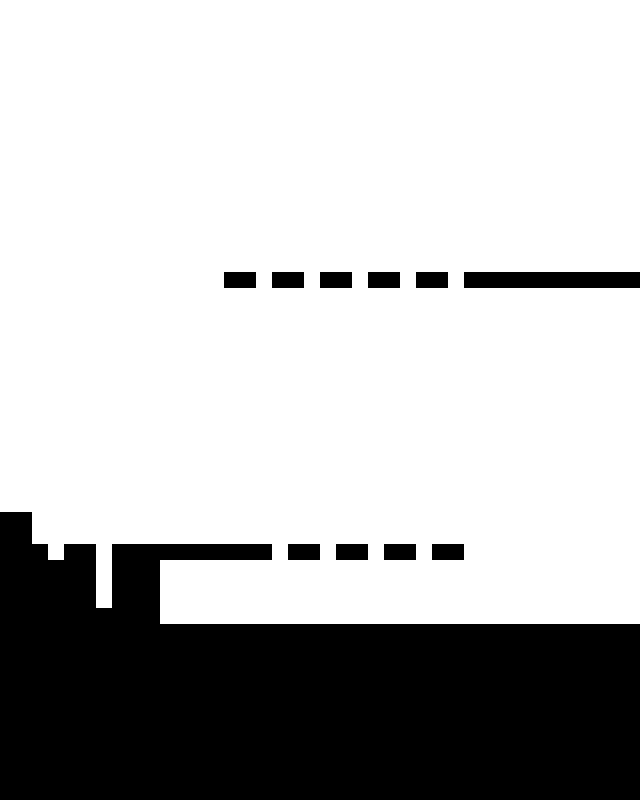
\includegraphics[width=0.50000\textwidth]{../data/super-mario-bros/generated/250n-3k-binary/image/105.png}
\caption{A binary spatial-style map based on \emph{Super Mario Bros.}
levels}\label{fig:mario-binary}
\end{figure}

\begin{figure}
\centering
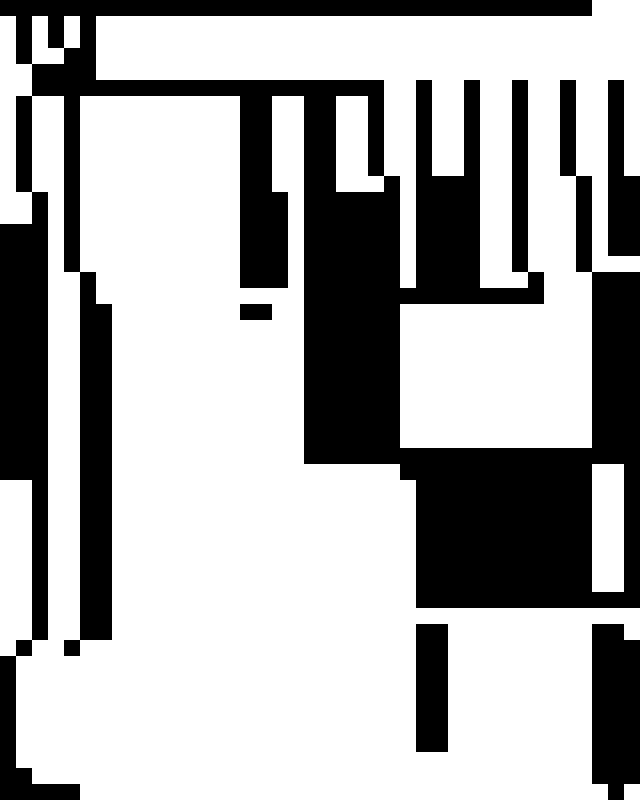
\includegraphics[width=0.50000\textwidth]{../data/pokemon-red/generated/250n-3k-binary/image/6.png}
\caption{A binary spatial-style map based on \emph{Pokemon Red}
maps}\label{fig:red-binary}
\end{figure}

\subsection{Backoff smoothing in 2d}\label{sec:backoff}

As explained before, backoff smoothing is useful when the Markov chain
encounters unknown states in the generated data; it allows us take less
predecessors into account when needed.

With linear Markov chains the backoff smoothing is easy to define: for
example, if we take three previous states into account usually, we can
take two instead. For 2d chains the problem is not so trivial since it
is not clear which elements we have to take and how many of them.

To facilitate our discussion we say that a predecessors matrix \(S\) is
a sub-matrix of predecessors matrix \(P\) if it satisfies the following
requirements:

\begin{itemize}
\tightlist
\item
  \(S\) must take less elements into account than \(P\)
\item
  \(S\) must not take into account elements that are at a larger
  distance than \(P\)
\end{itemize}

We can then simply implement backoff smoothing by taking a sub-matrix of
our current predecessors matrix. This is done in a recursive manner by
removing one element at the largest distance at a time. More formally,
the list of sub-matrices of a predecessor matrix \(P\) is given by:

\begin{equation}
subMatrices(P) \coloneqq\begin{cases}
\bigcup_{k \in K} subMatrices(k), & \text{if $k \neq 0$}.\\
0, & \text{otherwise}.
\end{cases}
\end{equation}

where \(K\) is the set of all matrices that are equal to \(P\) minus one
of the elements at the largest distance.

\begin{figure}[h]
\centering
$
\begin{pmatrix}
 0& 1& 2\\ 
 1& 1& 2\\ 
 2& 2& 2 
\end{pmatrix}
$
\caption{A matrix showing the notions of distance, each number gives the distance of the corresponding cell}
\end{figure}

\begin{figure}
\centering
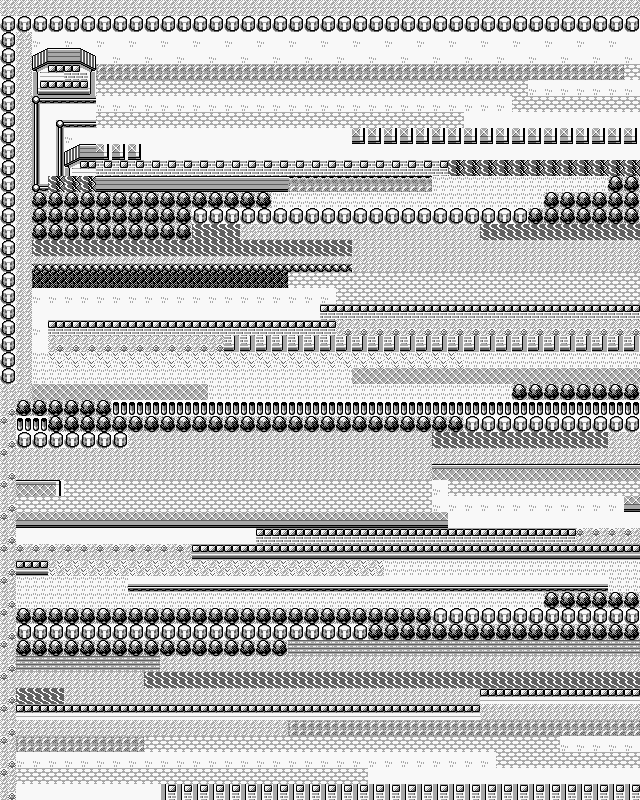
\includegraphics[width=0.50000\textwidth]{../data/pokemon-red/generated/250n-3k-without-backoff/image/12.png}
\caption{A \emph{Pokemon} map generated without backoff
smoothing.}\label{fig:backoff}
\end{figure}

In fig.~\ref{fig:backoff} we can see the results of a map generated
without backoff smoothing. The map starts off well with the house on the
upper left but then quickly degrades as soon it encounters a combination
of tiles that are not present in the training data. By mitigating this
effect backoff smoothing significantly improves the overall quality of
the generated maps. A drawback of the backoff smoothing method is that
it increases the computational time of both generation and training
exponentially with the size of the predecessors matrix. This implies
that in practice we cannot use very large predecessors matrices.

\section{Related work}\label{related-work}

Game companies generally do not publish their procedural content
generation methods so it is hard to evaluate what is common in the
industry. In academia, researchers have looked into various approaches
for automatic level generation. The game \emph{Super Mario Bros.} in
particular has received much attention.

Shaker et al. (2012) uses generative grammars combined with an
evolutionary algorithm to create \emph{Mario} levels that adapt
themselves to the player's experience. In another paper, Sorenson and
Pasquier (2010) also use an evolutionary algorithm to create a generic
framework for level creation. Their approach allows the level designer
to enforce multiple constraints on the generated levels making it
adaptable to multiple genres of games.

Rather than being evolutionary, our method draws from machine learning
techniques. The designers do not have to explicitly articulate rules
about their designs but simply need to provide the system with examples
of what they want to create.

Papers using machine learning methods to generate content are still a
minority, but the trend seems to be on the rise. Our use of Markov
chains is directly inspired by the work of Snodgrass and Ontañón (2013)
and Dahlskog, Togelius, and Nelson (2014). They both use Markov chains
to create \emph{Mario} levels with very convincing results. The
difference with our approach lies in the fact that \emph{Mario} levels
have a linear nature. The maps we focus on are non-linear; the player
can move through both dimensions. Additionally we use maps with a much
higher number of tiles: \emph{Pokemon red} has a total number of 125
unique tiles, \emph{Pokemon FireRed} has 1207 unique tiles, in contrast
the maps used by Snodgrass and Ontañón (2013) have only 11 unique tiles.
Our sample is more representative of modern games in which the
technological constraints limiting the number of unique tiles have
almost disappeared.

Adam J Summerville and Mateas (2015) explore non-linear level generation
in the context of dungeons for the game \emph{The Legend of Zelda}.
Their use of a graph to represent the game space comes from Dormans
(2010). Our focus is more on world maps rather than dungeons. Dungeons
have a clear compartmentalization of individual rooms while world maps
have a more organic unfolding of space. Furthermore, dungeons have
elements such as locked doors that restrict the order in which the
player can traverse the rooms. World maps typically do not have these
types of constraints.

Finally, the video game level corpus provided by Adam James Summerville
et al. (2016) supplied us with the necessary data to generate
\emph{Super Mario Bros} maps.

\section{Conclusion and further research}\label{sec:conclusion}

While not perfect, our method shows that Markov chains have potential
for the generation of non-linear maps particularly when the number of
unique tiles is relatively small.

There are many ways our method could improved:

\begin{itemize}
\tightlist
\item
  We could create quantitative measures of map quality, generate a large
  number of them and then select only the best. Since maps can be
  created relatively fast this should be feasible, the only drawback
  being that it is hard to define measures of map quality that are
  independent of the game being used.
\item
  We could find ways of grouping semantically similar tiles into the
  same high-level concepts and thus reduce the total number of unique
  tiles in the tile-maps.
\item
  Instead of using 2d Markov chains, we could use Markov random fields
  (Murphy 2012). Their main difference with Markov chains lies in the
  fact that they encode dependencies between their elements in a
  non-sequential way. Since we want to create non-linear maps they might
  be better suited for the task. The disadvantage of using Markov random
  fields comes from the fact that they are harder to implement and they
  both require more time to train and to sample appropriately.
\end{itemize}

Our approach is not restricted to games and we can easily imagine using
this method with 3D models composed of voxels. Tiles would be replaced
by voxels and the Markov chains would be extended to work in 3d.

In the end though, machine learning techniques for content generation
have inherent limits that make the removal of human intervention not
conceivable at the moment:

\begin{itemize}
\tightlist
\item
  All the data used for training is created by humans, we cannot expect
  to use these methods in areas where data is scarce or non-existent.
\item
  Machine learning techniques have a hard time capturing high-level
  themes, their creations make sense at a local scale but fail to
  reproduce the holistic feel of the training data. In the case of a
  game, levels are often organized with the intention of teaching a
  player a new gameplay mechanic. For example, the underlying theme of a
  \emph{Mario} level could be showing the player how to handle flying
  enemies, all the level would be built around this motif. A data-driven
  algorithm trained on all the available levels in \emph{Mario} would
  mix data from thematically different levels and thus fail to
  accurately portray the intention of the designers. In theory this
  problem could be solved by having a separate dataset for each possible
  theme in a game, in practice though, designers only create one example
  for each theme which is clearly not sufficient.
\end{itemize}

In conclusion, we do not see these methods as a replacement for the
designer but rather as a tool, taking over in the most repetitive parts
of the work. The designer is then free to focus on what really matters:
transmitting his creative vision.

\section*{References}\label{references}
\addcontentsline{toc}{section}{References}

\hypertarget{refs}{}
\hypertarget{ref-Dahlskog2014}{}
Dahlskog, Steve, Julian Togelius, and Mark J. Nelson. 2014. ``Linear
levels through n-grams.'' \emph{Proceedings of the 18th International
Academic MindTrek Conference on Media Business, Management, Content \&
Services - AcademicMindTrek '14}, 200--206.
doi:\href{https://doi.org/10.1145/2676467.2676506}{10.1145/2676467.2676506}.

\hypertarget{ref-Dormans2010}{}
Dormans, Joris. 2010. ``Adventures in level design: generating missions
and spaces for action adventure games.'' \emph{\ldots{} Workshop on
Procedural Content Generation in Games}, 1--8.
doi:\href{https://doi.org/10.1145/1814256.1814257}{10.1145/1814256.1814257}.

\hypertarget{ref-Lindenmayer1968}{}
Lindenmayer, a. 1968. ``Mathematical models for cellular interactions in
development. II. Simple and branching filaments with two-sided inputs.''
\emph{Journal of Theoretical Biology} 18 (3): 300--315.
doi:\href{https://doi.org/10.1016/0022-5193(68)90080-5}{10.1016/0022-5193(68)90080-5}.

\hypertarget{ref-Murphy2012}{}
Murphy, Kevin P. 2012. \emph{Machine learning: a probabilistic
perspective}. MIT press.

\hypertarget{ref-Shaker2012}{}
Shaker, Noor, Miguel Nicolau, Georgios N. Yannakakis, Julian Togelius,
and Michael O'Neill. 2012. ``Evolving levels for Super Mario Bros using
grammatical evolution.'' \emph{2012 IEEE Conference on Computational
Intelligence and Games, CIG 2012}, no. 1: 304--11.
doi:\href{https://doi.org/10.1109/CIG.2012.6374170}{10.1109/CIG.2012.6374170}.

\hypertarget{ref-Snodgrass2013}{}
Snodgrass, Sam, and Santiago Ontañón. 2013. ``Generating Maps Using
Markov Chains.'' \emph{Aiide}, 25--28.
\url{http://www.aaai.org/ocs/index.php/AIIDE/AIIDE13/paper/viewPDFInterstitial/7447/7632}.

\hypertarget{ref-Sorenson2010}{}
Sorenson, Nathan, and Philippe Pasquier. 2010. ``Towards a Generic
Framework for Automated Video Game Level Creation Applications of
Evolutionary Computation'' 6024: 131--40 ST--Towards a Generic Framework
for Auto.
doi:\href{https://doi.org/10.1007/978-3-642-12239-2_14}{10.1007/978-3-642-12239-2\_14}.

\hypertarget{ref-Summerville2015}{}
Summerville, Adam J, and Michael Mateas. 2015. ``The Learning of Zelda :
Data-Driven Learning of Level Topology,'' no. Fdg.

\hypertarget{ref-Summerville2016}{}
Summerville, Adam James, Sam Snodgrass, Michael Mateas, and Santiago
Ontañón. 2016. ``The VGLC: The Video Game Level Corpus.'' \emph{Arxiv}.
\url{http://arxiv.org/abs/1606.07487}.

\end{document}
